\documentclass[tikz, border=10pt]{standalone}
\usepackage[utf8]{inputenc}
\usepackage{tikz}
\usetikzlibrary{shapes.geometric, arrows.meta, positioning, fit, backgrounds}

\definecolor{kept}{RGB}{210,225,245}
\definecolor{changed}{RGB}{255,224,178}
\definecolor{newnode}{RGB}{198,239,206}
\definecolor{future}{RGB}{235,235,235}

\tikzset{
  block/.style={rectangle, rounded corners, minimum width=6.6cm, minimum height=1.05cm,
    text centered, draw=black, align=center, font=\small},
  futureblock/.style={rectangle, rounded corners, minimum width=5.4cm, minimum height=1.0cm,
    text centered, draw=black, dashed, align=center, font=\scriptsize, fill=future},
  arrowline/.style={thick, -{Stealth[length=3mm]}},
  dashedline/.style={thick, dashed, -{Stealth[length=3mm]}, red!70!black},
  futureline/.style={thick, dashed, -{Stealth[length=2.5mm]}, gray}
}

\begin{document}
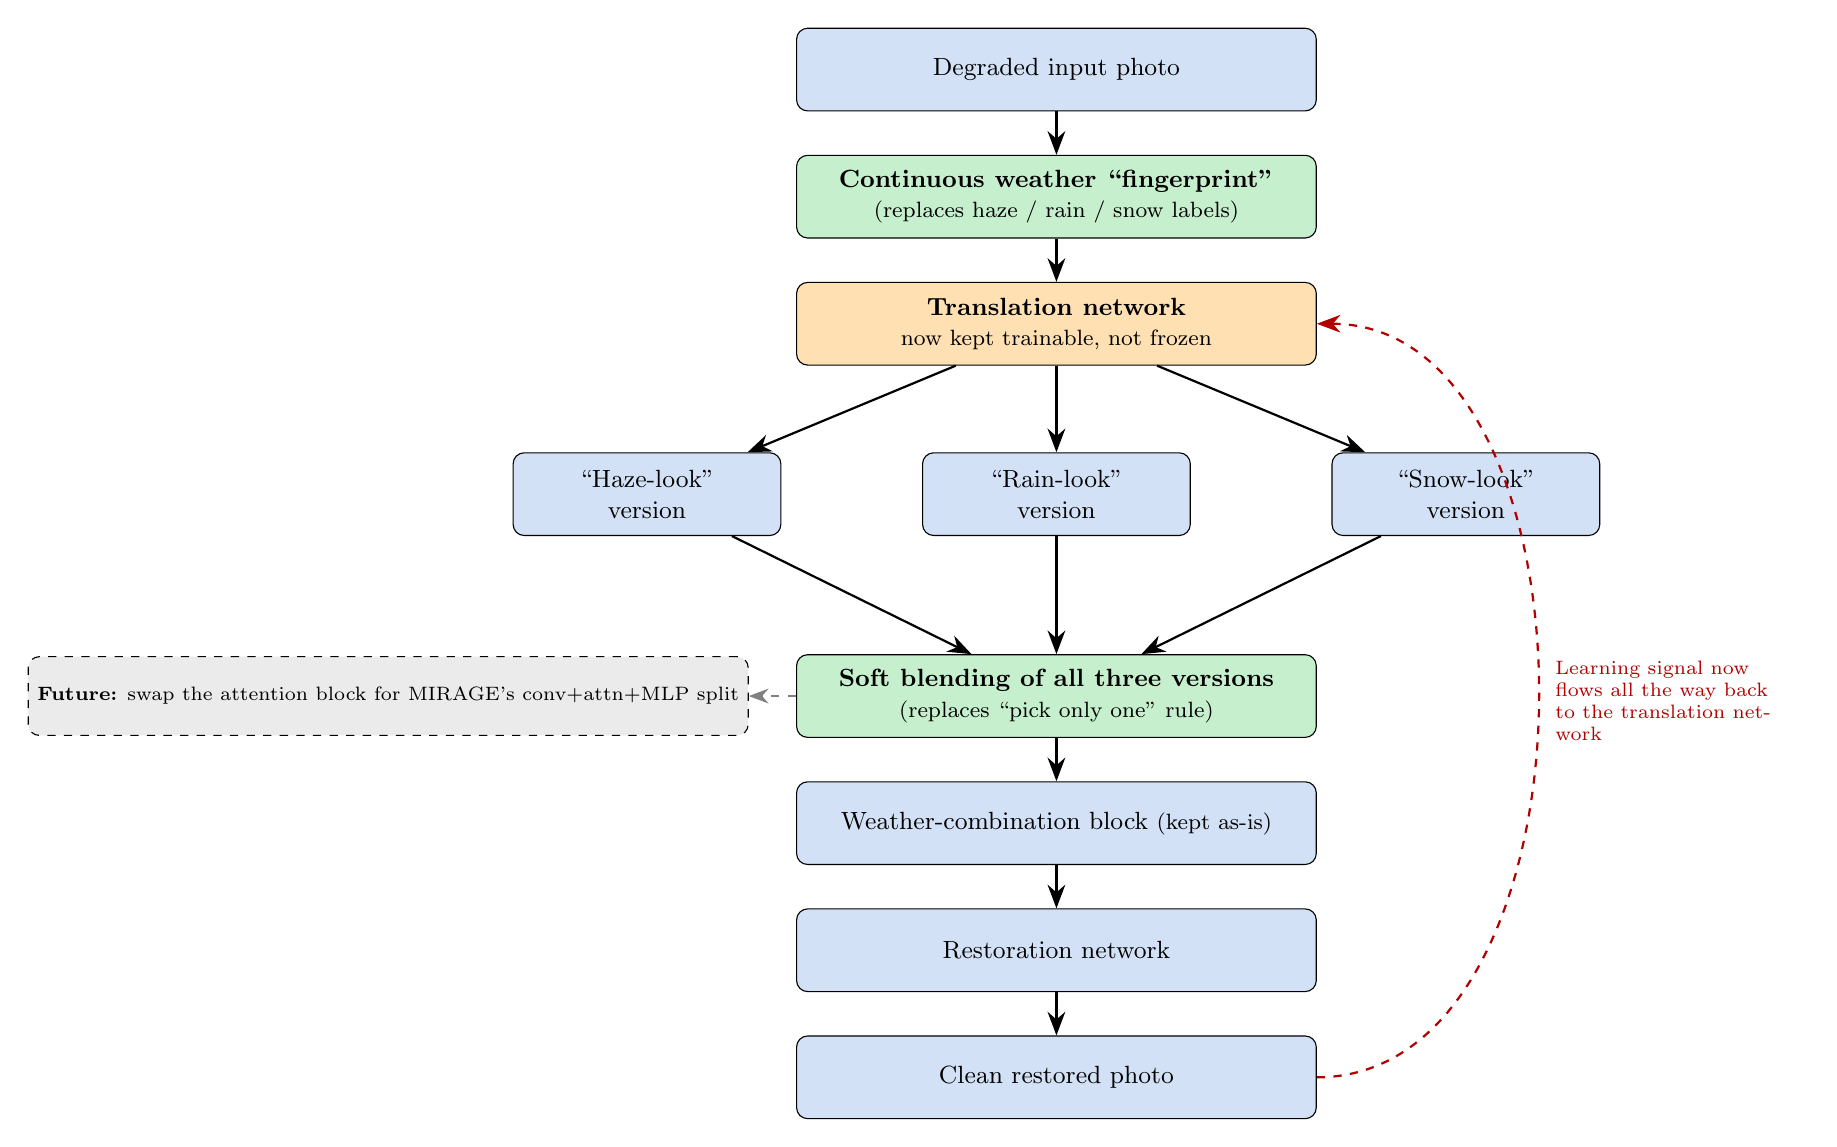
\begin{tikzpicture}[node distance=0.55cm]
\node[block, fill=kept] (input) {Degraded input photo};
\node[block, fill=newnode, below=of input] (embed)
  {\textbf{Continuous weather ``fingerprint''}\\ \footnotesize (replaces haze / rain / snow labels)};
\node[block, fill=changed, below=of embed] (translate)
  {\textbf{Translation network}\\ \footnotesize now kept trainable, not frozen};
\node[block, fill=kept, minimum width=3.4cm, below=1.1cm of translate, xshift=-5.2cm] (haze) {``Haze-look''\\version};
\node[block, fill=kept, minimum width=3.4cm, below=1.1cm of translate, xshift=0cm] (rain) {``Rain-look''\\version};
\node[block, fill=kept, minimum width=3.4cm, below=1.1cm of translate, xshift=5.2cm] (snow) {``Snow-look''\\version};
\node[block, fill=newnode, below=1.5cm of rain] (routing)
  {\textbf{Soft blending of all three versions}\\ \footnotesize (replaces ``pick only one'' rule)};
\node[block, fill=kept, below=of routing] (fusion) {Weather-combination block \footnotesize (kept as-is)};
\node[block, fill=kept, below=of fusion] (restore) {Restoration network};
\node[block, fill=kept, below=of restore] (output) {Clean restored photo};

\node[futureblock, left=0.6cm of routing] (ext1)
  {\textbf{Future:} swap the attention block for MIRAGE's conv+attn+MLP split};

\draw[arrowline] (input) -- (embed);
\draw[arrowline] (embed) -- (translate);
\draw[arrowline] (translate) -- (haze);
\draw[arrowline] (translate) -- (rain);
\draw[arrowline] (translate) -- (snow);
\draw[arrowline] (haze) -- (routing);
\draw[arrowline] (rain) -- (routing);
\draw[arrowline] (snow) -- (routing);
\draw[arrowline] (routing) -- (fusion);
\draw[arrowline] (fusion) -- (restore);
\draw[arrowline] (restore) -- (output);

\draw[dashedline] (output.east) to[out=0,in=0] node[right, xshift=1mm, font=\scriptsize, text width=3.1cm, align=left]
  {Learning signal now flows all the way back to the translation network} (translate.east);
\draw[futureline] (routing.west) -- (ext1.east);
\end{tikzpicture}
\end{document}
